\section{Auswertung}
\label{sec:Auswertung}
Die Fehler der Widerstände $R$, Kapazitäten $C$ und der Induktivitäten $I$ betragen jeweils $\pm \qty{0.2}{\percent}$. Das Verhältnis $R3/R4$ am Potentiometer
weist einen Fehler von $\pm \qty{0.5}{\percent}$ auf und die verstellbaren Widerstände eine Ungenauigkeit von $\pm \qty{3}{\percent}$. 

\subsection{Wheatstonesche Brücke}
\label{subsec:wheat_aus}
\begin{table}[H]
  \centering
  \caption{Messwerte der Wheatstoneschen Brücke.}
  \label{tab:wheat}
  \sisetup{table-format=3.0}
  \begin{tabular}{S[table-format=4.0] S S S[table-format=3.2]}
   \toprule
    {$R_2 $[\si{\ohm}]} & {$R_3$ [\si{\ohm}]} & {$R_4 $[\si{\ohm}]}&{ $R_x = Wert10$[\si{\ohm}]}\\
   \midrule
   332 & 420 & 580 & 240.41 \\
   500 & 325 & 675 &  240.74\\
   1000 & 194 & 806 &  240.70\\
   \bottomrule
  \end{tabular}
\end{table} 

Für die Berechnung des Mittelwerts 
\begin{equation*}
  R_{\text{xm}} = 240.62
\end{equation*}
und der Standardabweichung
\begin{equation*}
  \sigma_{\text{xm}} = 0.14
\end{equation*}
von $R_x$ wurde das Pythonmodul Numpy \cite{numpy} herangezogen.
Der Fehler des Mittelwerts berechnet sich analog zu
\begin{equation*}
  \Delta R_{\text{xm}}= 0.08.
\end{equation*}

\noindent Die Fehlerfortpflanzung nach Gauß, gemäß
\begin{equation*}
  \Delta f = \sqrt{\biggl(\frac{\partial f}{\partial x}\biggr)^2\cdot (\Delta x)^2 + \biggl(\frac{\partial f}{\partial y}\biggr)^2\cdot (\Delta y)^2 +
  \cdots + \biggl(\frac{\partial f}{\partial z}\biggr)^2\cdot (\Delta z)^2}
\end{equation*}
wird im folgenden auch mithilfe des Pythonmoduls Numpy \cite{numpy} berechnet.
\subsection{Kapazitätsmessbrücke}
\label{subsec:kap_aus}
\begin{table}[H]
  \centering
  \caption{Messwerte der Kapazitätsmessbrücke.}
  \label{tab:kap}
  \sisetup{table-format=3.0}
  \begin{tabular}{c S S S S S[table-format=3.2] S[table-format=3.2]}
   \toprule
  &{$C_2$ [\si{\nano\farad}]}&{$R_2$ [\si{\ohm}]} & {$R_3$ [\si{\ohm}]} & {$R_4$ [\si{\ohm}]}&{$R_x$ [\si{\ohm}]} & {$C_x$ [\si{\nano\farad}]}\\
  \midrule
   Wert 9 & 992 & 192 & 691 & 309 & 443.6 & 429.36\\
   Wert 1 & 992 & 0 & 605 & 395 & 647.67 & 0 \\
   \bottomrule
  \end{tabular}
\end{table}


  

\subsection{Induktivitätsmessbrücke}
\label{subsec:indu_aus}
\begin{table}[H]
  \centering
  \caption{Messwerte der Induktivitätsmessbrücke.}
  \label{tab:indu}
  \sisetup{table-format=3.0}
  \begin{tabular}{c S S S S S[table-format=3.2] S[table-format=3.2]}
  \toprule
  &{$L_2$ [\si{\milli\henry}]}&{$R_2$ [\si{\ohm}]} & {$R_3$ [\si{\ohm}]} & {$R_4$ [\si{\ohm}]}&{$R_x$ [\si{\ohm}]} & {$L_x$ [\si{\milli\henry}]}\\
  \midrule
  Wert 17& 27.5 & 59 & 609 & 391 & 91.90 & 42.83\\
  \bottomrule
  \end{tabular}
\end{table}
Die Fehler der 

Wien-Robinson-Brücke
\begin{figure}
  \centering
  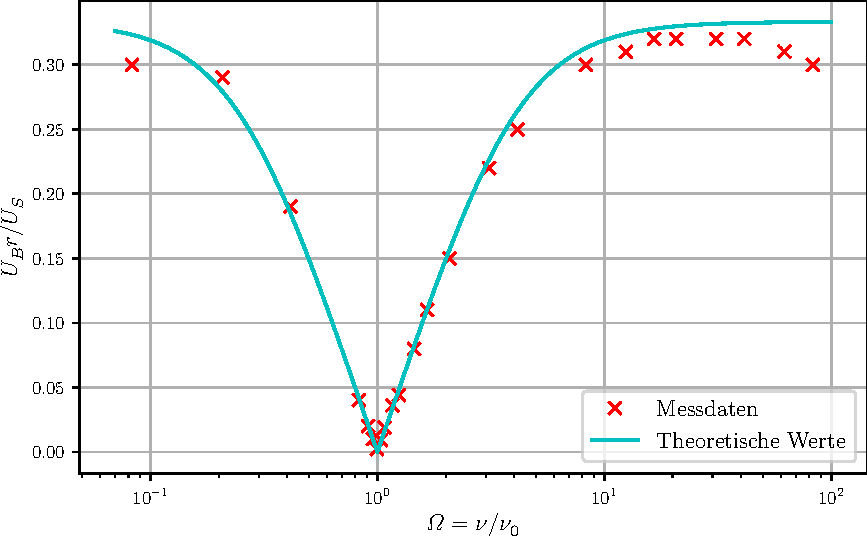
\includegraphics{plot.pdf}
  \caption{keine Ahnung wie man das nennt...}
  \label{fig:wrb-plot}
\end{figure}



